\documentclass[a4paper, 12pt]{article}
\usepackage{config}

\begin{document}
	\begin{center}
		\begin{huge}
			Resumo dos Comandos
		\end{huge}
	\end{center}

	\begin{itemize}
		\item Lista de comandos a ser tratada
		\begin{itemize}
			\item\ttt{Plot}
			\item\ttt{Plot3D}
			\item\ttt{ContourPlot}
			\item \ttt{ParametricPlot}
			\item\ttt{StreamPlot}
			\item\ttt{VectorPlot}
			\item\ttt{Show}
		\end{itemize}
	\end{itemize}

	\section{Plot}
	Normal recebe uma função que depende de somente uma variável seguida da definição do intervalo de amostragem desejado. Então imagine que se deseja plotar a função do segundo $f(x)=x^{2}$, para fazer isso basta tomar o lado direito da função e utilizar como primeiro parâmetro do \ttt{Plot} como segue.	

	\begin{lstlisting}[language=Mathematica]
	Plot[x^2]
	\end{lstlisting}
	
	Porém, não é adequado parar por aqui, é necessário definir a variação de $x$ em uma dimensão que vai abranger o ``teatro'' escolhido. Dessa maneira, imagine que queiramos plotar essa função de modo a abranger os valores de $x$ que vão de -1 a 1, então aplicamos \ttt{\{x,-1,1\}}. Como consequência, percebe-se que o programa lança valores de $x$ abrangendo o domínio explicitado de modo a conformar a representação gráfica no menor espaço possível de visualização do gráfico para os valores de $x$ propostos
	
	\begin{lstlisting}[language=Mathematica]
	Plot[x^2,{x,-1,1}]
	\end{lstlisting}
	
	Da forma como está, se dermos \ttt{enter} o comando será rodado e vamos obter
	
	\begin{figure}[!h]\label{parabola}
		\centering
		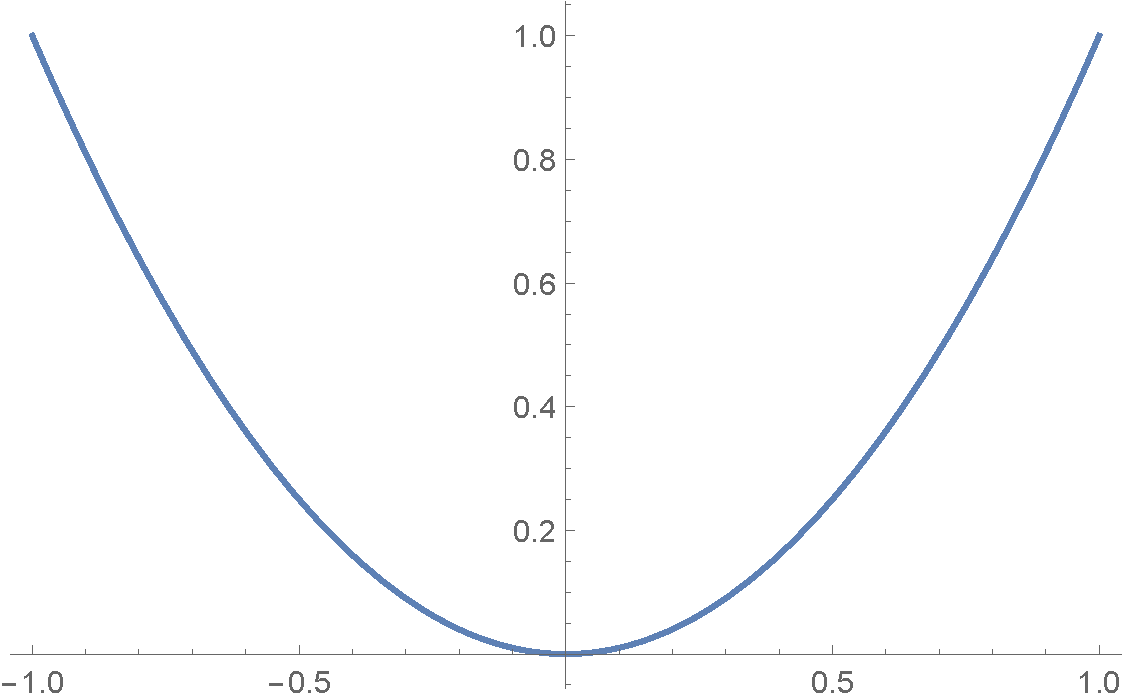
\includegraphics[scale=.5]{images/parabola}
	\end{figure}

	Repare que sendo $x=-1$ ou $x=1$, $f(x)=1$, logo o máximo valor de $f$ mostrado é 1, não precisamos a variação de $y$, até mesmo por que o \ttt{Plot} não aceitaria tal sintaxe. 
	
	\section{Plot3D}
	Podemos interpretar esse comando como expansão do \ttt{Plot}, porém em três dimensões. Sabendo que um ponto no espaço agora depende de $x$ e $y$, consequentemente a função $f(x)$ em duas dimensões passará a ser $f(x,y)$. De forma análoga ao que foi feito para o comando anterior, imagine que queiramos plotar um paraboloide no espaço que obedeça
	
	\begin{equation}
		f(x,y)=x^2+y^2
	\end{equation}
	
	Numa abordagem rápida, podemos imaginar tal superfície como a rotação de uma parábola tal como é visto em \ref{parabola} em torno do eixo $z$ no espaço, então sabendo que dependemos de mais uma variável será preciso acrescentar outro parâmetro ao \ttt{Plot3D} como segue
	
	\begin{lstlisting}[language=Mathematica]
	Plot3D[x^2+y^2,{x,-1,1},{y,-1,1}]
	\end{lstlisting}
	
	\begin{figure}[!h]\label{parabola}
		\centering
		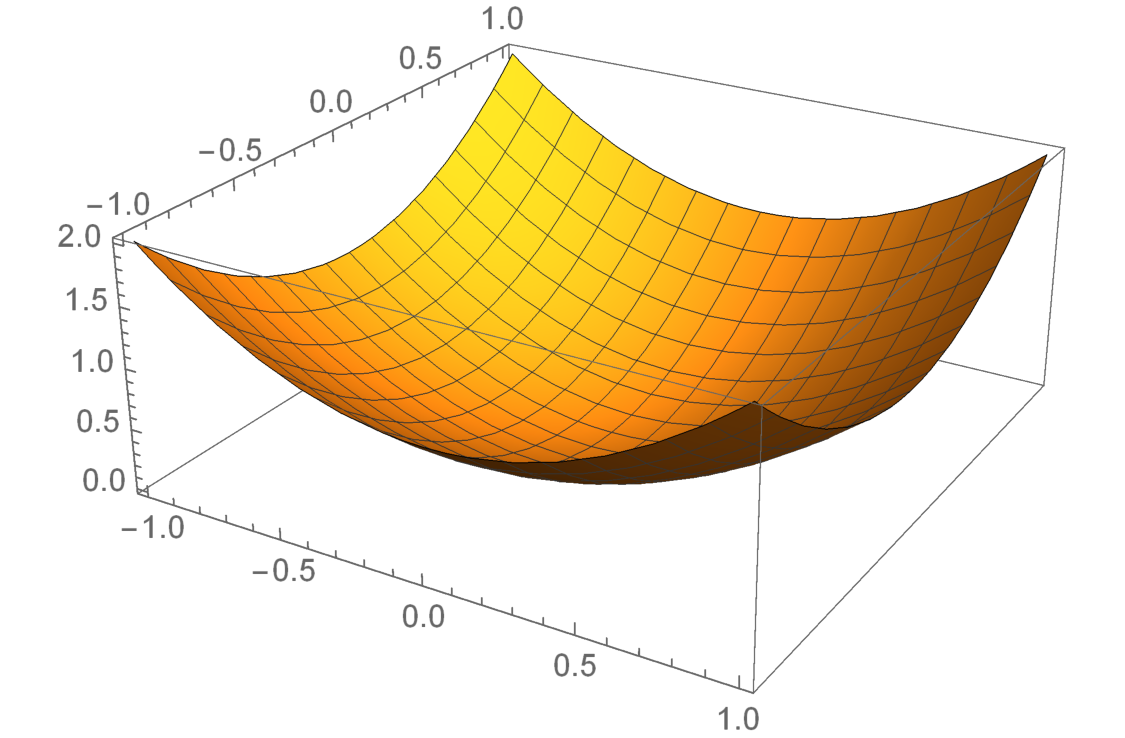
\includegraphics[scale=.6]{images/parabola3d}
	\end{figure}

	Note que se clicarmos com o botão direito do \textit{mouse} e formos na opção \textit{Top View} veremos
	
	\begin{figure}[!h]\label{parabola}
		\centering
		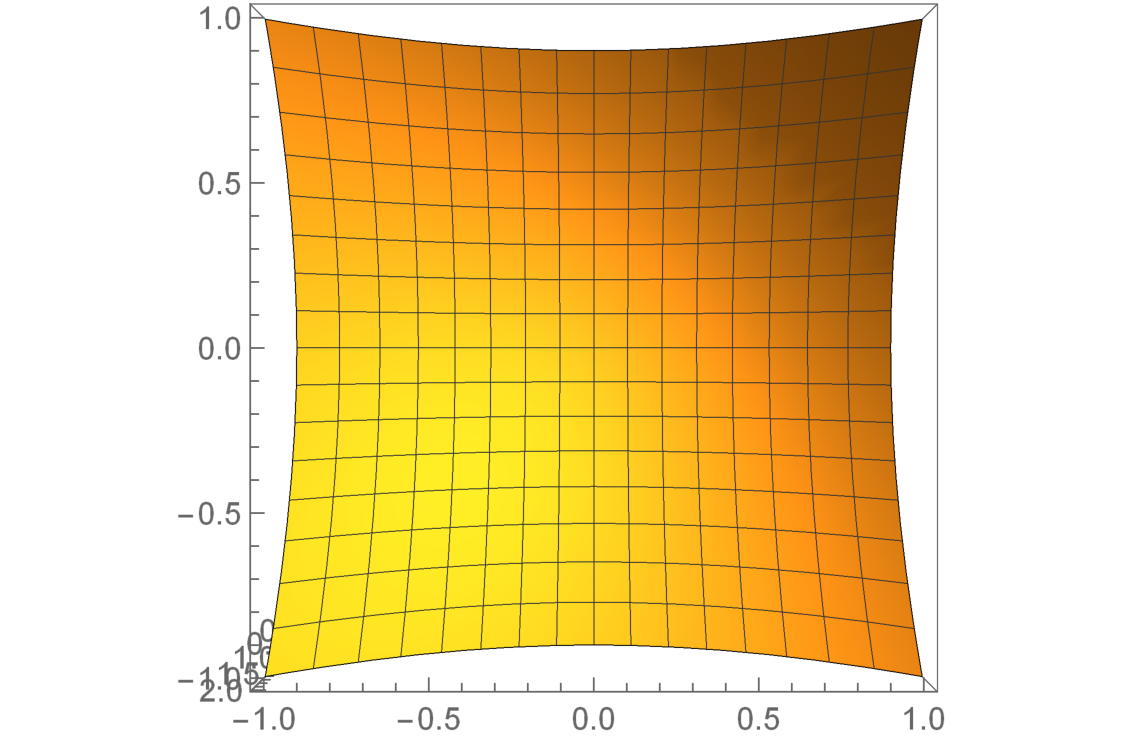
\includegraphics[scale=.55]{images/parabola3dtop}
	\end{figure}
	
	Ou seja, o intervalo de valores escolhido para $x$ e $y$ novamente é notado no domínio presente. Vê-se que a vista superior é um quadrado de lados valendo 2 unidades já que tanto $x$ quanto $y$ variam entre menos -1 e 1.
	
	Partindo para análise em $z$, vamos mudar a opção de \textit{Top View} para \textit{Front View}. Fazendo uma análise visual vemos que a máxima altura da ``caixa'' que comporta o gráfico é de duas unidades. Isso ocorre pois o máximo valor que $f(x,y)$ pode assumir para o domínio escolhido ocorre quando as coordenadas são $(-1,-1)$, $(-1,1)$, $(1,-1)$ ou $(1,1)$ como vemos a seguir
	
	\begin{figure}[!h]\label{parabola}
		\centering
		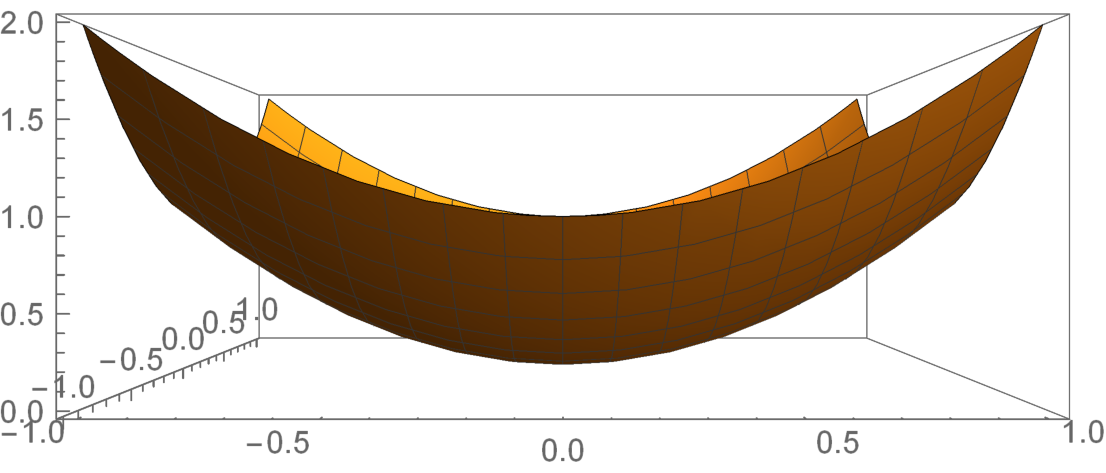
\includegraphics[scale=.55]{images/parabola3dfront}
	\end{figure}

	Sabemos disso devido a simplicidade do gráfico e prevemos que a função é sempre crescente no intervalo dado.
	
	Alguns atributos de estilo podem ser passados para os \ttt{Plot}s de modo a melhorar a visualização ou visando cumprir alguma meta de representação gráfica. Alguns dos comandos a seguir são interessantes de serem entendidos pelo menos no básico.
	
	\vspace{.5cm}
	Para o \ttt{Plot} (Gráficos em 2d no geral) 
	\begin{itemize}
		\item\ttt{AspectRatio}
		\begin{itemize}
			\item Permite editar a proporção entre os eixos do gráfico. Imagine que quiséssemos uma proporção de 1 em $x$ para dois em $y$, teríamos uma razão igual a 0.5 e podemos prever que o gráfico terá maior comprimento em $x$ que em $y$ como vemos a seguir com base nas linhas de comando
		\end{itemize}
	
\begin{lstlisting}[language=Mathematica]
Plot[x^2,{x,-1,1},AspectRatio -> .5]
\end{lstlisting}
		
		\begin{figure}[!h]\label{parabola}
			\centering
			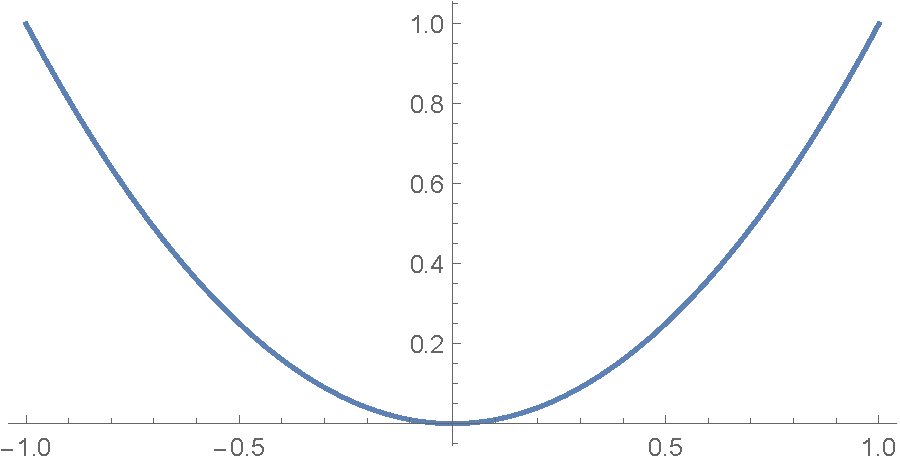
\includegraphics[scale=.55]{images/aspecthalf}
		\end{figure}
		
		Trocando por 2 o valor da propriedade vemos
		
\begin{lstlisting}[language=Mathematica]
Plot[x^2,{x,-1,1},AspectRatio -> 2]
\end{lstlisting}
		
		\newpage 
		\begin{figure}[!h]\label{parabola}
			\centering
			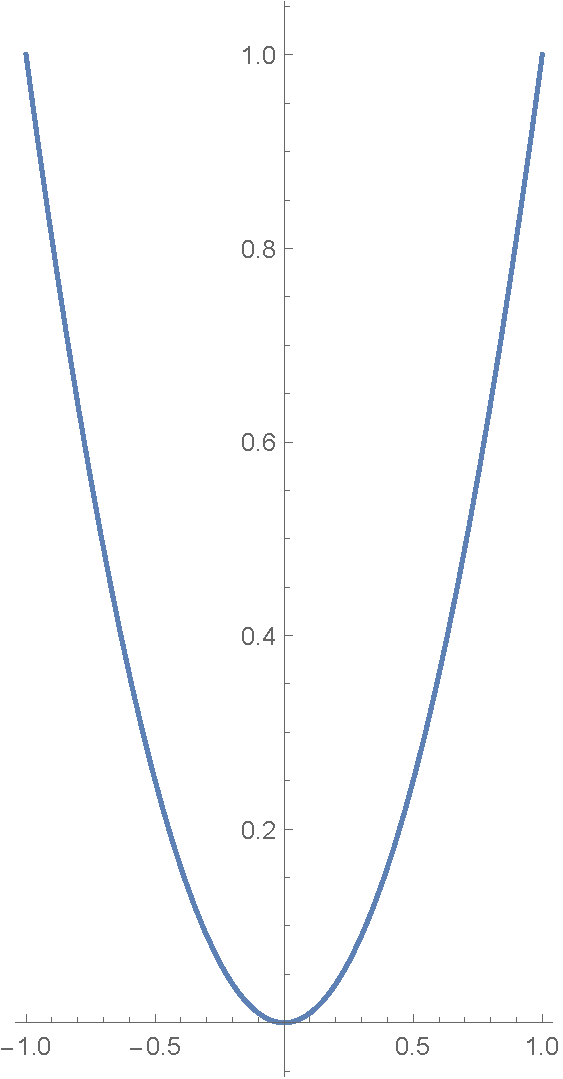
\includegraphics[scale=.55]{images/aspectdouble}
		\end{figure}
	
		\item\ttt{PlotStyle} 
			\begin{itemize}
				\item Um dos atributos mais utilizados, possibilita mudar a cor do gráfico, espessura das linhas, opacidade, entre muitos outros parâmetros. 
				\begin{itemize}
					\item Mudando a cor
					\begin{itemize}
						\item Uma maneira aconselhável é passar diretamente o atributo de cor, como por exemplo \ttt{Magenta}, \ttt{Red}, \ttt{Blue}, \ttt{Cyan} ou utilizar o \ttt{RGBColor} para customizar com maior liberdade como segue
					\end{itemize}
				\end{itemize}
			\end{itemize}
		
\begin{lstlisting}[language=Mathematica]
Plot[x^2,{x,-1,1},AspectRatio -> .5,PlotStyle -> Magenta]
\end{lstlisting}

\begin{figure}[!h]\label{parabola}
	\centering
	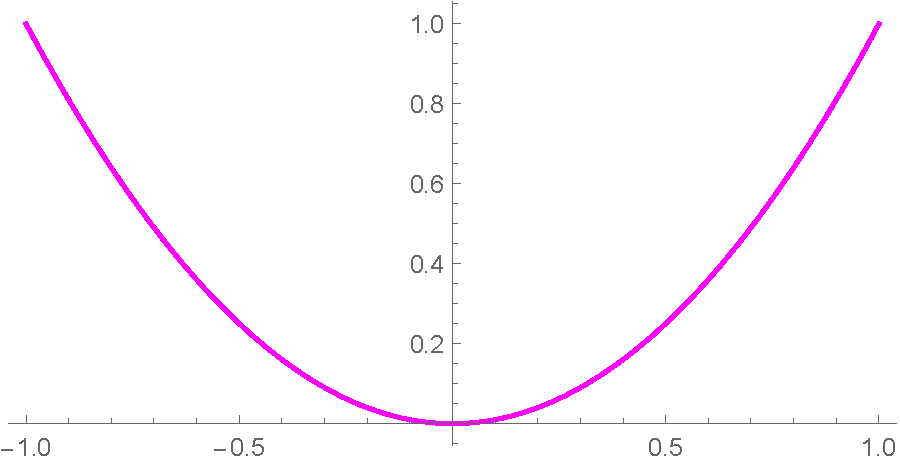
\includegraphics[scale=.55]{images/magenta}
\end{figure}

		\item\ttt{GridLines} 
		\begin{itemize}
			\item Nos permite adicionar uma malha quadriculada ao fundo da plotagem. Esse recurso muitas vezes facilita a associação entre os eixos coordenados e nos permite ter maior precisão quantitativa para aproximações feitas visualmente. Abaixo temos alguns exemplos.
		\end{itemize}


\begin{lstlisting}[language=Mathematica]
Plot[x^2,{x,-1,1},AspectRatio->.5,PlotStyle->Magenta,GridLines->Automatic]
\end{lstlisting}
\begin{figure}[!h]\label{parabola}
	\centering
	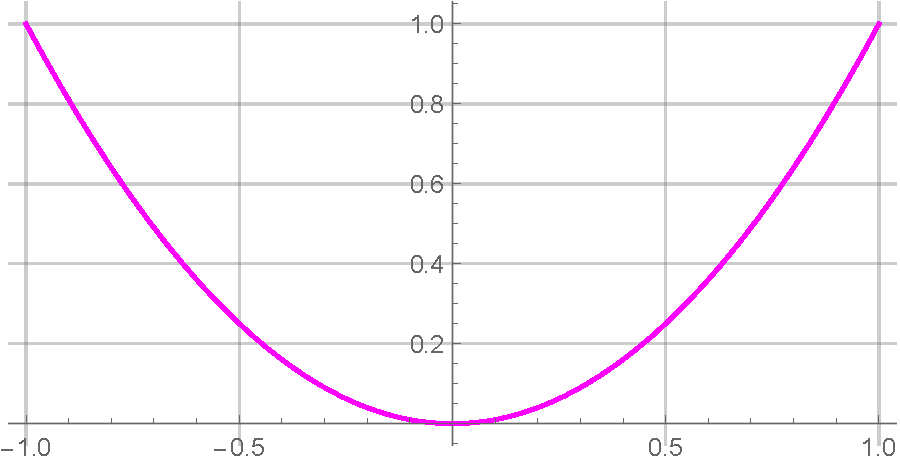
\includegraphics[scale=.55]{images/grid}
\end{figure}
		
		\begin{itemize}
			\item[] Por padrão o \ttt{GridLines} com \ttt{Automatic} renderiza linhas cheias, mas podemos alterálas passando \ttt{GridLinesStyle->\{\{Dashed\},\{Dashed\}\}}. Isso fará com que tanto as linha horizontais quanto as verticais se tornem tracejadas. De forma semelhante usamos o \ttt{Dotted} para deixá-las pontilhadas. O atributo de cor também pode ser passado no interior das chaves como vemos a seguir
		\end{itemize}

\begin{lstlisting}[language=Mathematica]
Plot[x^2,{x,-1,1},AspectRatio->.5,PlotStyle->Magenta,GridLines->Automatic,GridLinesStyle->{{Red, Dotted, Thick},{Gray, Dotted}}}]
\end{lstlisting}
\begin{figure}[!h]\label{parabola}
	\centering
	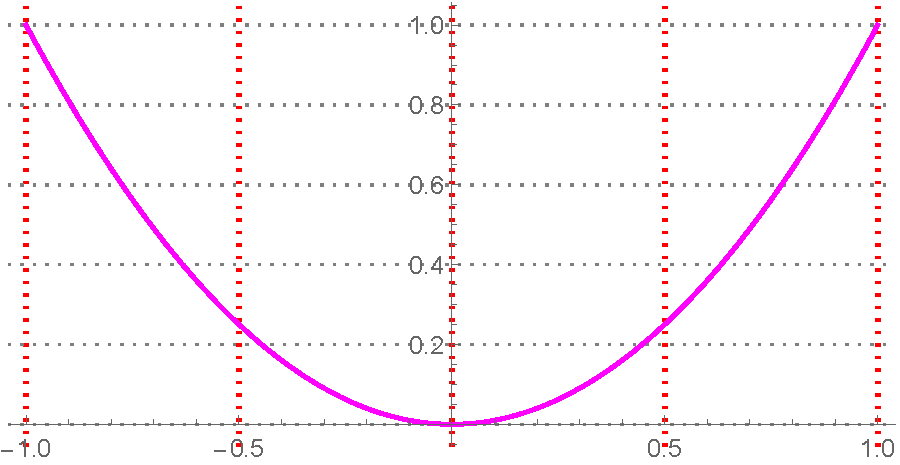
\includegraphics[scale=.85]{images/gridStyle}
\end{figure}

	\begin{itemize}
		\item[] Aumentando-se a proporção do gráfico vê-se que a primeira lista de valores contendo \ttt{Red}, \ttt{Dotted} e \ttt{Thick} tornou as linhas verticais vermelhas, pontilhadas e, como foi passado o \ttt{Thick} houve uma leve aumentada na espessura, somente para melhorar a visualização do leitor.
	\end{itemize}

	\end{itemize}

	\newpage
	\vspace{.5cm}
	Para o \ttt{Plot3D} (Gráficos em 3d no geral) 
	\begin{itemize}
		\item\ttt{BoxRatios}
		\begin{itemize}
			\item Esse atributo é análogo ao \ttt{AspectRatio}, porém fazemos sua aplicação para três dimensões com base numa lista de três posições indicando a proporção em cada eixo como segue
			
\begin{lstlisting}[language=Mathematica]
Plot3D[x^2+y^2,{x,-1,1},{y,-1,1},BoxRatios->{1,1,1}]
\end{lstlisting}
			\begin{figure}[!h]
				\centering
				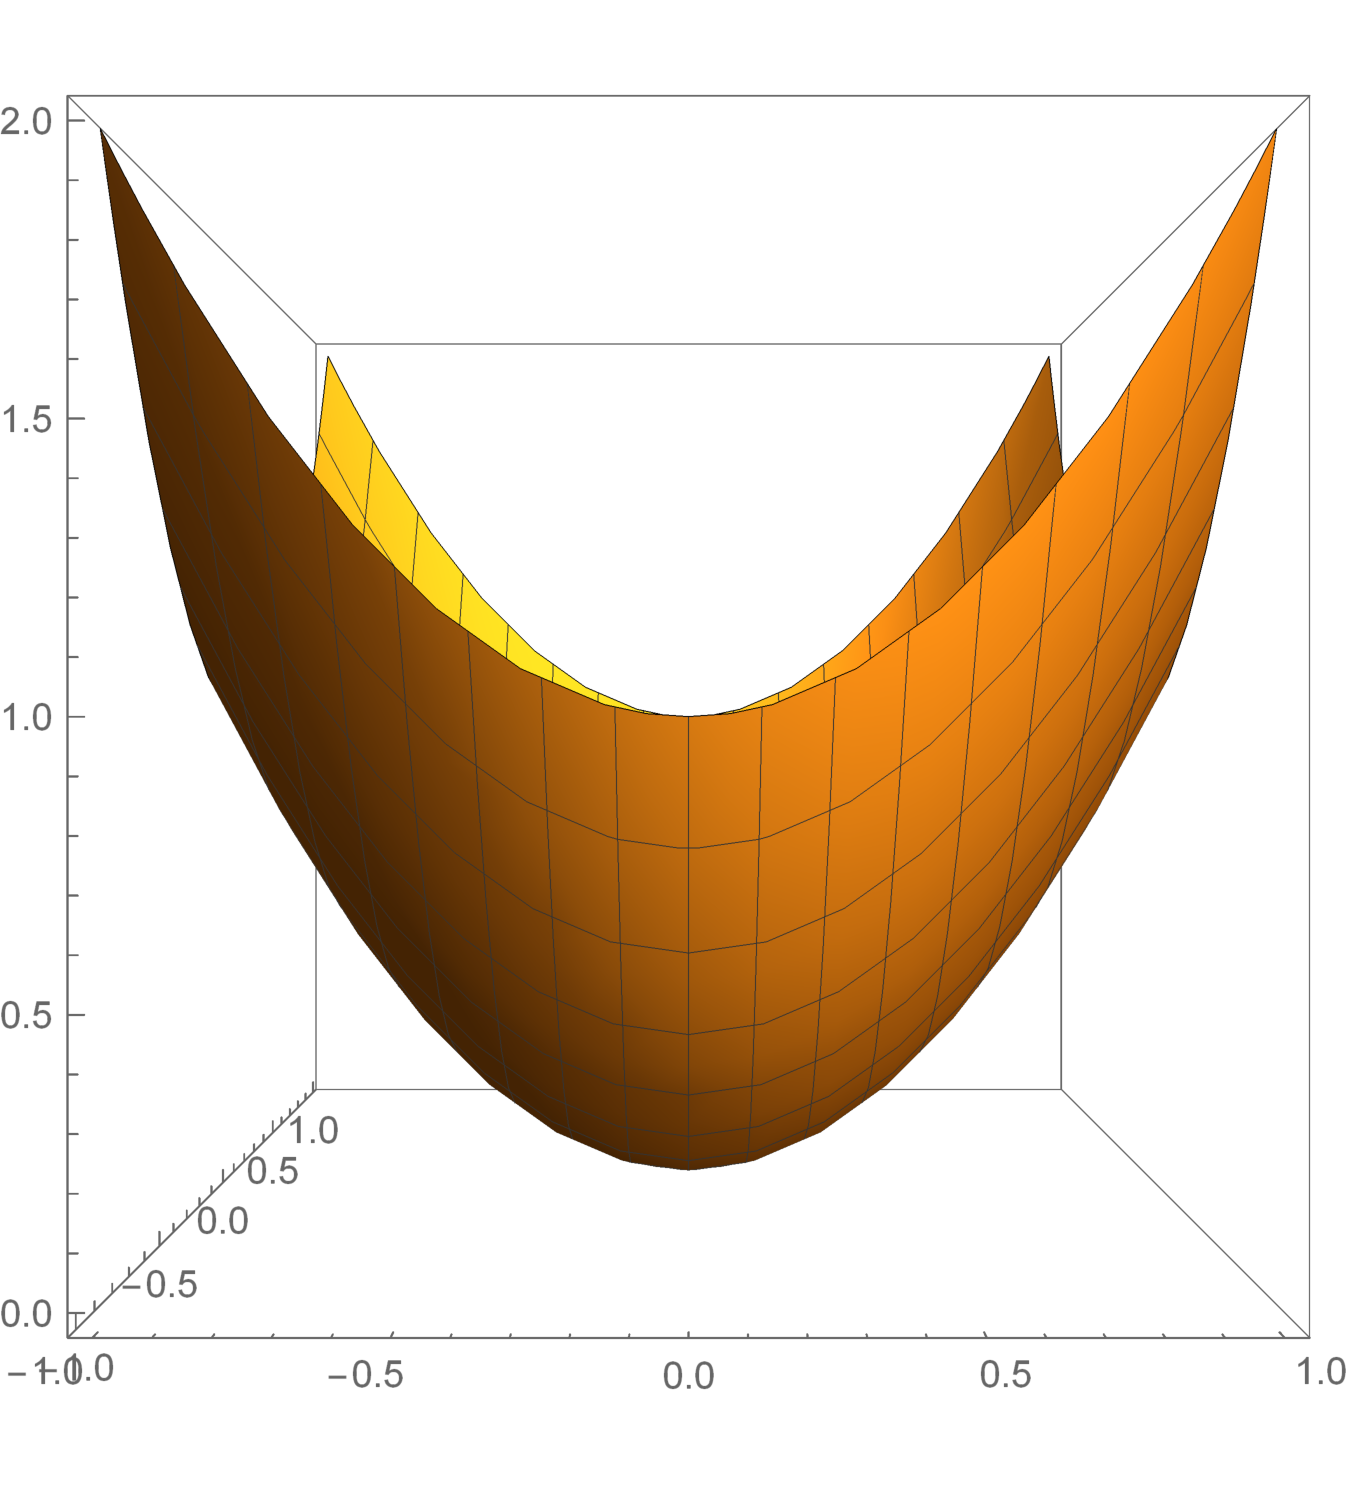
\includegraphics[scale=.35]{images/boxRatios}
			\end{figure}
			Como é visto, a proporção do gráfico foi aumentada ocasionando um estreitamento de sua base e aumento de sua altura na escala. 
			
			Caso quiséssemos testar fazer uma figura com o eixo $z$ com metade da proporção, note a diferença

\begin{lstlisting}[language=Mathematica]
Plot3D[x^2+y^2,{x,-1,1},{y,-1,1},BoxRatios->{1,1,.5}]
\end{lstlisting}

		\begin{figure}[!h]
			\centering
			\includegraphics[scale=.35]{images/metadeboxRatios}
		\end{figure}

		\end{itemize}
		\item\ttt{Filling}
		\begin{itemize}
			\item Ferramenta bastante útil na estilização dos gráficos, nos permite criar um sombreado preenchendo a parte inferior das superfícies. Também é aplicável no \ttt{Plot}
			
\begin{lstlisting}[language=Mathematica]
Plot3D[x^2+y^2,{x,-1,1},{y,-1,1},Filling->Bottom]
\end{lstlisting}
			
			\begin{figure}[!h]
				\centering
				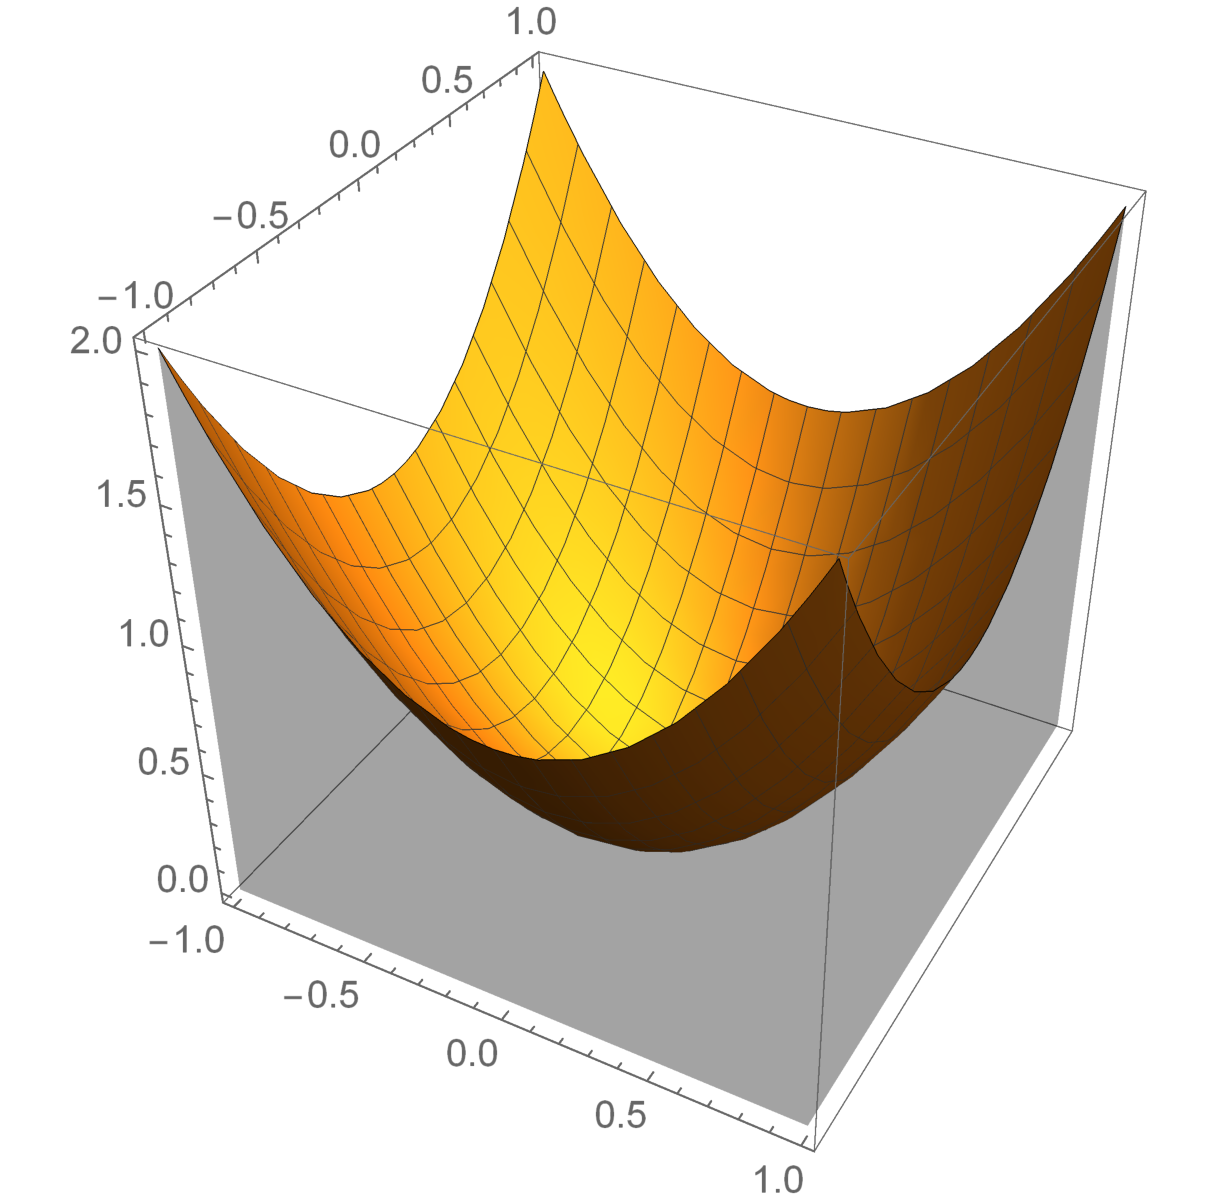
\includegraphics[scale=.45]{images/Filling}
			\end{figure}
			
			\begin{itemize}
				\item Aplicando o \ttt{FillingStyle}, até então não mencionado podemos obter
\begin{lstlisting}[language=Mathematica]
Plot3D[x^2+y^2,{x,-1,1},{y,-1,1},Filling->Bottom,FillingStyle->Opacity[.8],PlotStyle->Red]
\end{lstlisting}

				\begin{figure}[!h]
					\centering
					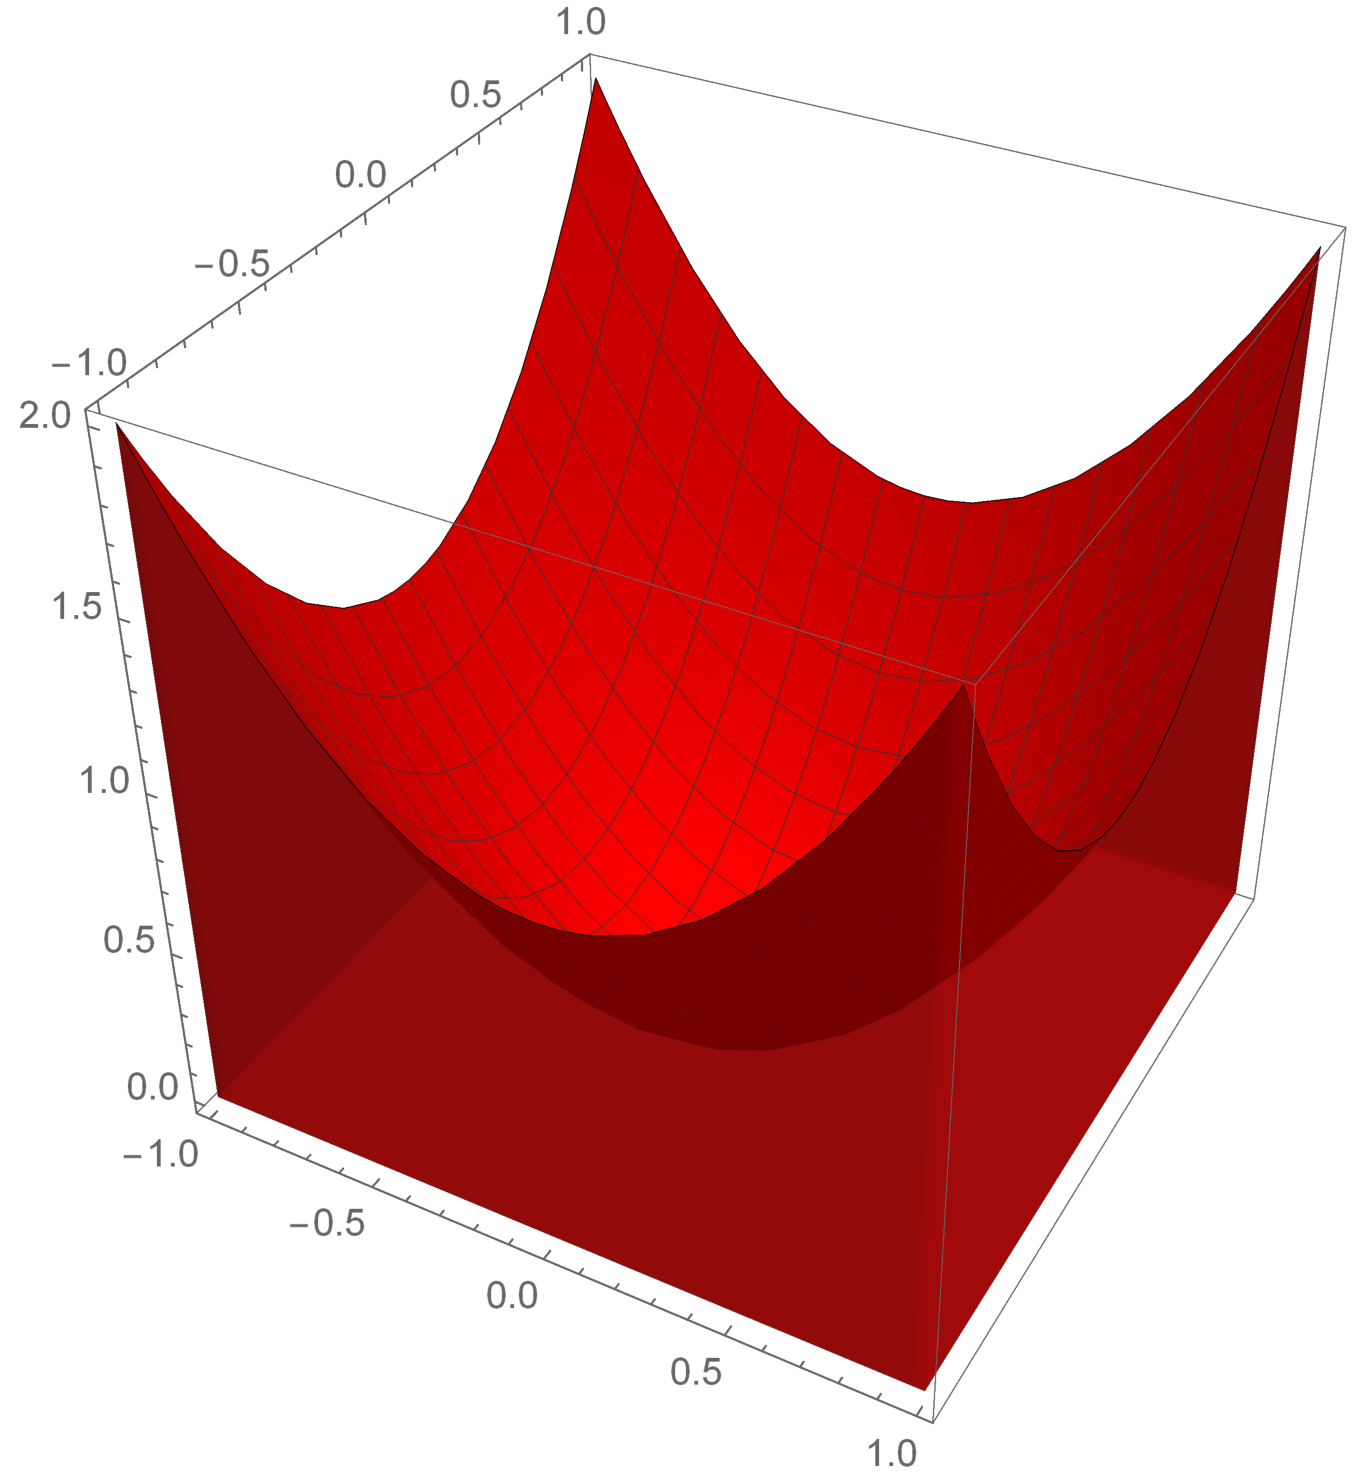
\includegraphics[scale=.45]{images/FillingStyle}
				\end{figure}
			\end{itemize}
		
		\end{itemize}
		\item\ttt{BoundaryStyle}
		
			Cria um contorno ao longo das bordas da superfície.
\begin{lstlisting}[language=Mathematica]
Plot3D[x^2+y^2,{x,-1,1},{y,-1,1},BoundaryStyle->{Thick,RGBColor[0,255,255]}]
\end{lstlisting}
			
			\begin{figure}[!h]
				\centering
				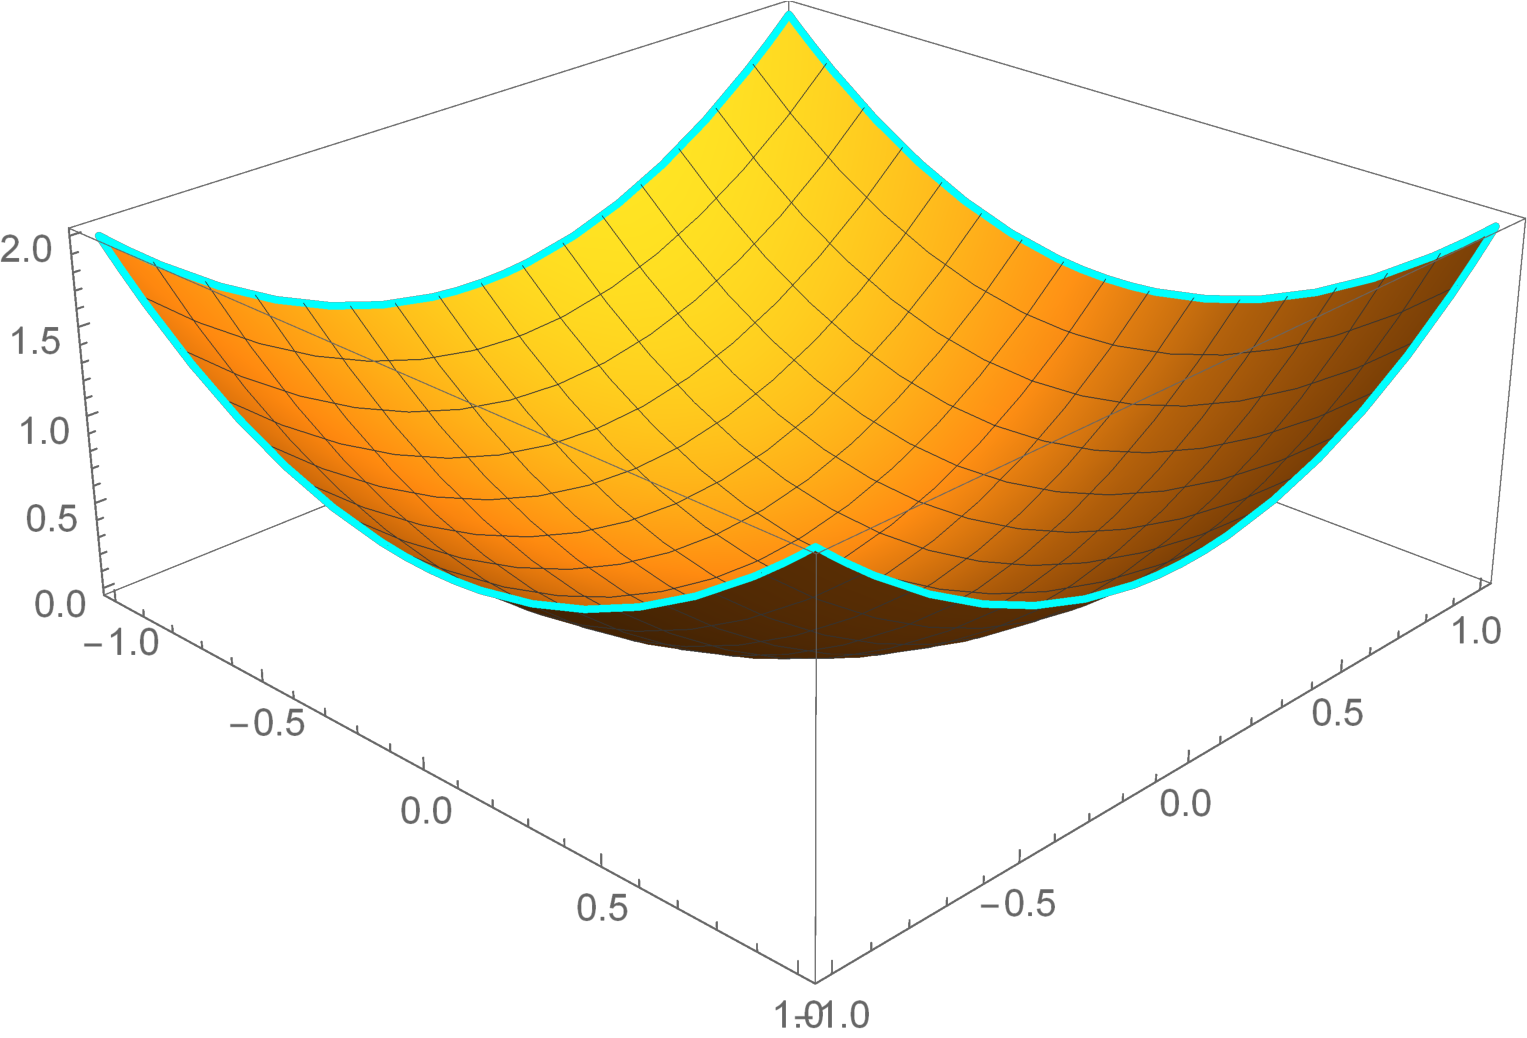
\includegraphics[scale=.45]{images/BoundaryStyle}
			\end{figure}
		\item\ttt{PlotStyle}
			
			Vamos resgatar algumas propriedades de estilização já conhecidas mostrando alguns exemplos de superfícies 

\begin{lstlisting}[language=Mathematica]
Plot3D[x^3 + y^3, {x, -1, 1}, {y, -1, 1}, PlotStyle -> {Green}, 
BoundaryStyle -> {Thick, Blue}, Filling -> Bottom, 
FillingStyle -> {Opacity[.2]}, BoxRatios -> {1, 1, 3}]
\end{lstlisting}

			\begin{figure}[!h]
				\centering
				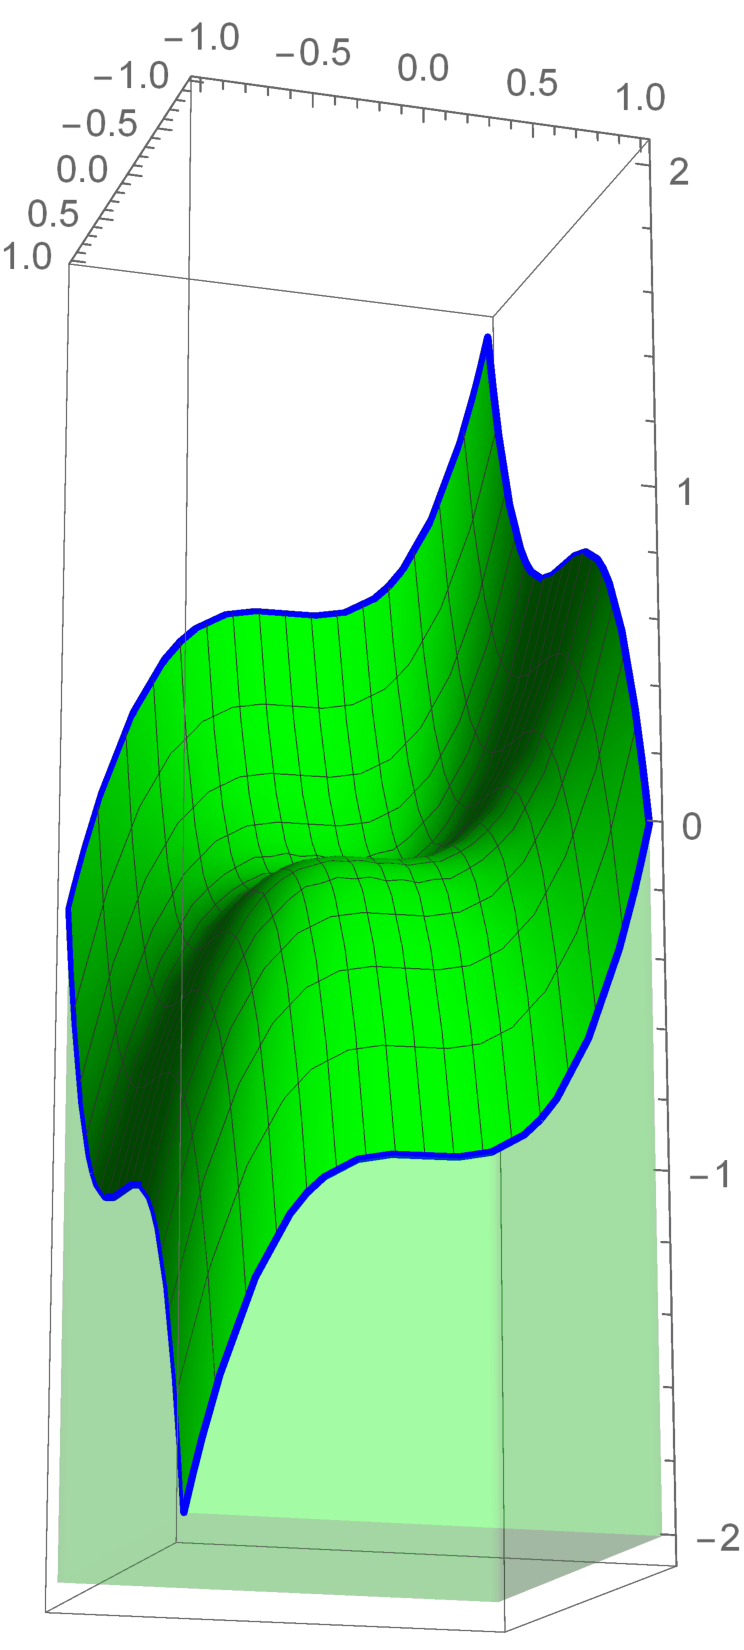
\includegraphics[scale=.3]{images/PlotStyle3d2}
			\end{figure}

\begin{lstlisting}[language=Mathematica]
Plot3D[x^2 + y^2, {x, -1, 1}, {y, -1, 1}, PlotStyle -> {LightBlue},BoundaryStyle -> {Thick, Blue}, Filling -> Bottom,FillingStyle -> {Opacity[.2]}]
\end{lstlisting}

			\begin{figure}[!h]
				\centering
				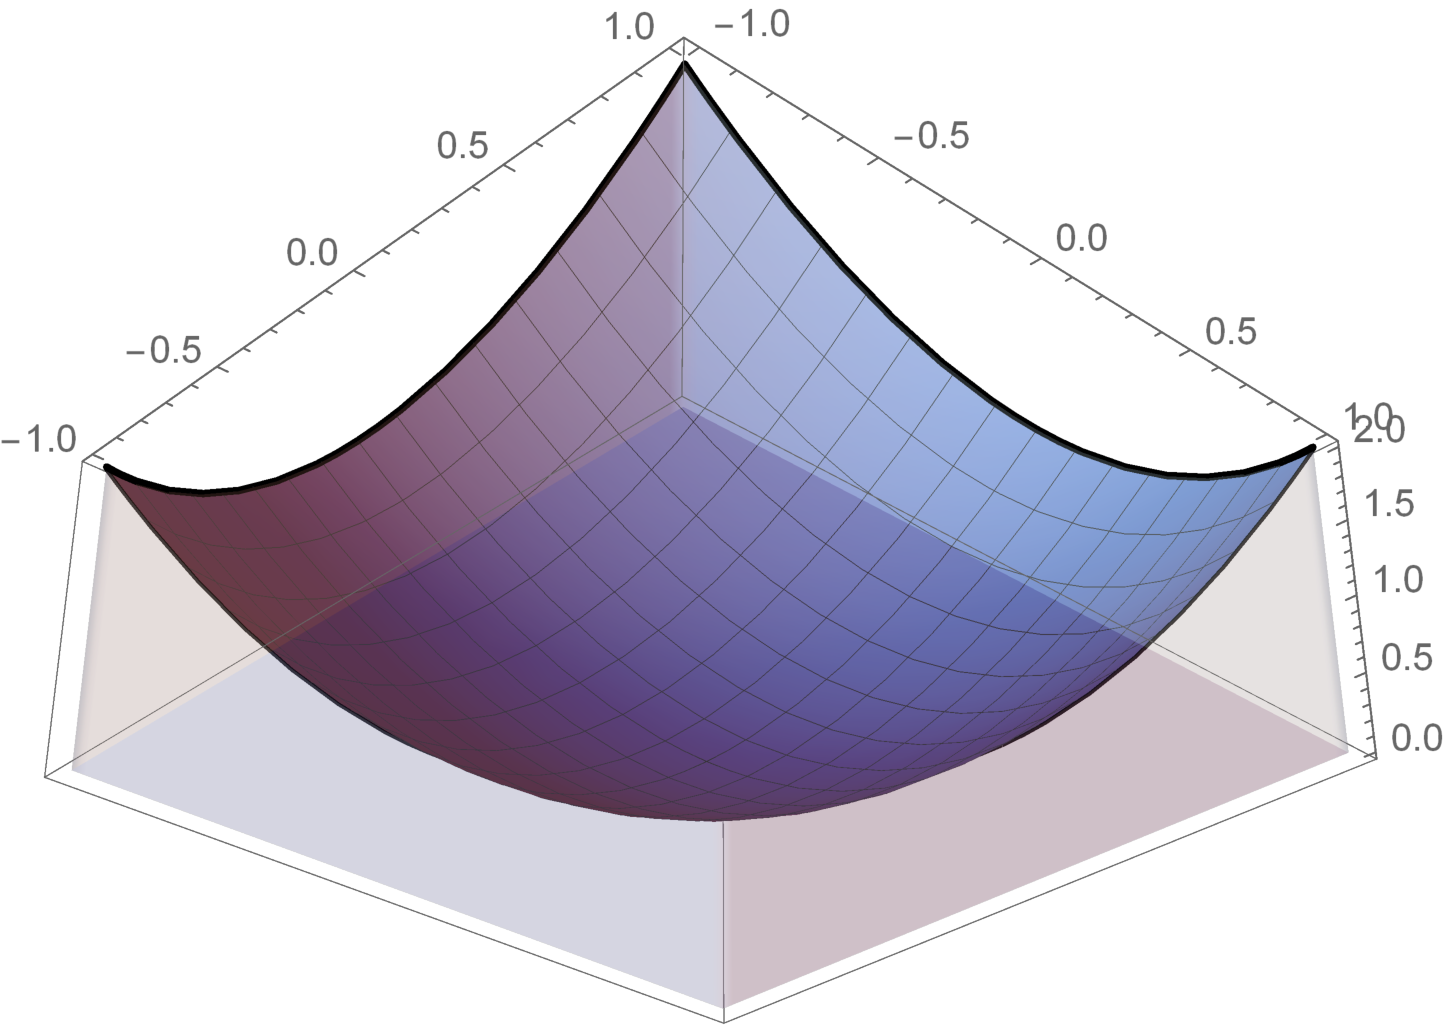
\includegraphics[scale=.5]{images/PlotStyle3d1}
			\end{figure}
	\end{itemize}

	\section{ContourPlot}
		Esse comando nos permite plotar os contornos de funções a depender de como passamos os parâmetros. Podemos imaginar que caso passarmos uma expressão seguindo a mesma estrutura do \ttt{Plot} vamos ter a replicação da função $f$ ao longo do eixo $y$ em diferentes alturas. Vamos exemplificar para tornar mais fácil.
		
		Imagine que desejamos novamente plotar a função do segundo grau $f(x)=x^{2}$, só que dessa vez, ao invés de plotar somente uma curva queremos uma família de funções que seguem o mesmo molde porém transladadas em $y$. Dessa forma, passaríamos o comando como é visto abaixo 
		
\begin{lstlisting}[language=Mathematica]
ContourPlot[y - x^2, {x, -1, 1}, {y, -1, 1}]
\end{lstlisting}

\begin{figure}[!h]
	\centering
	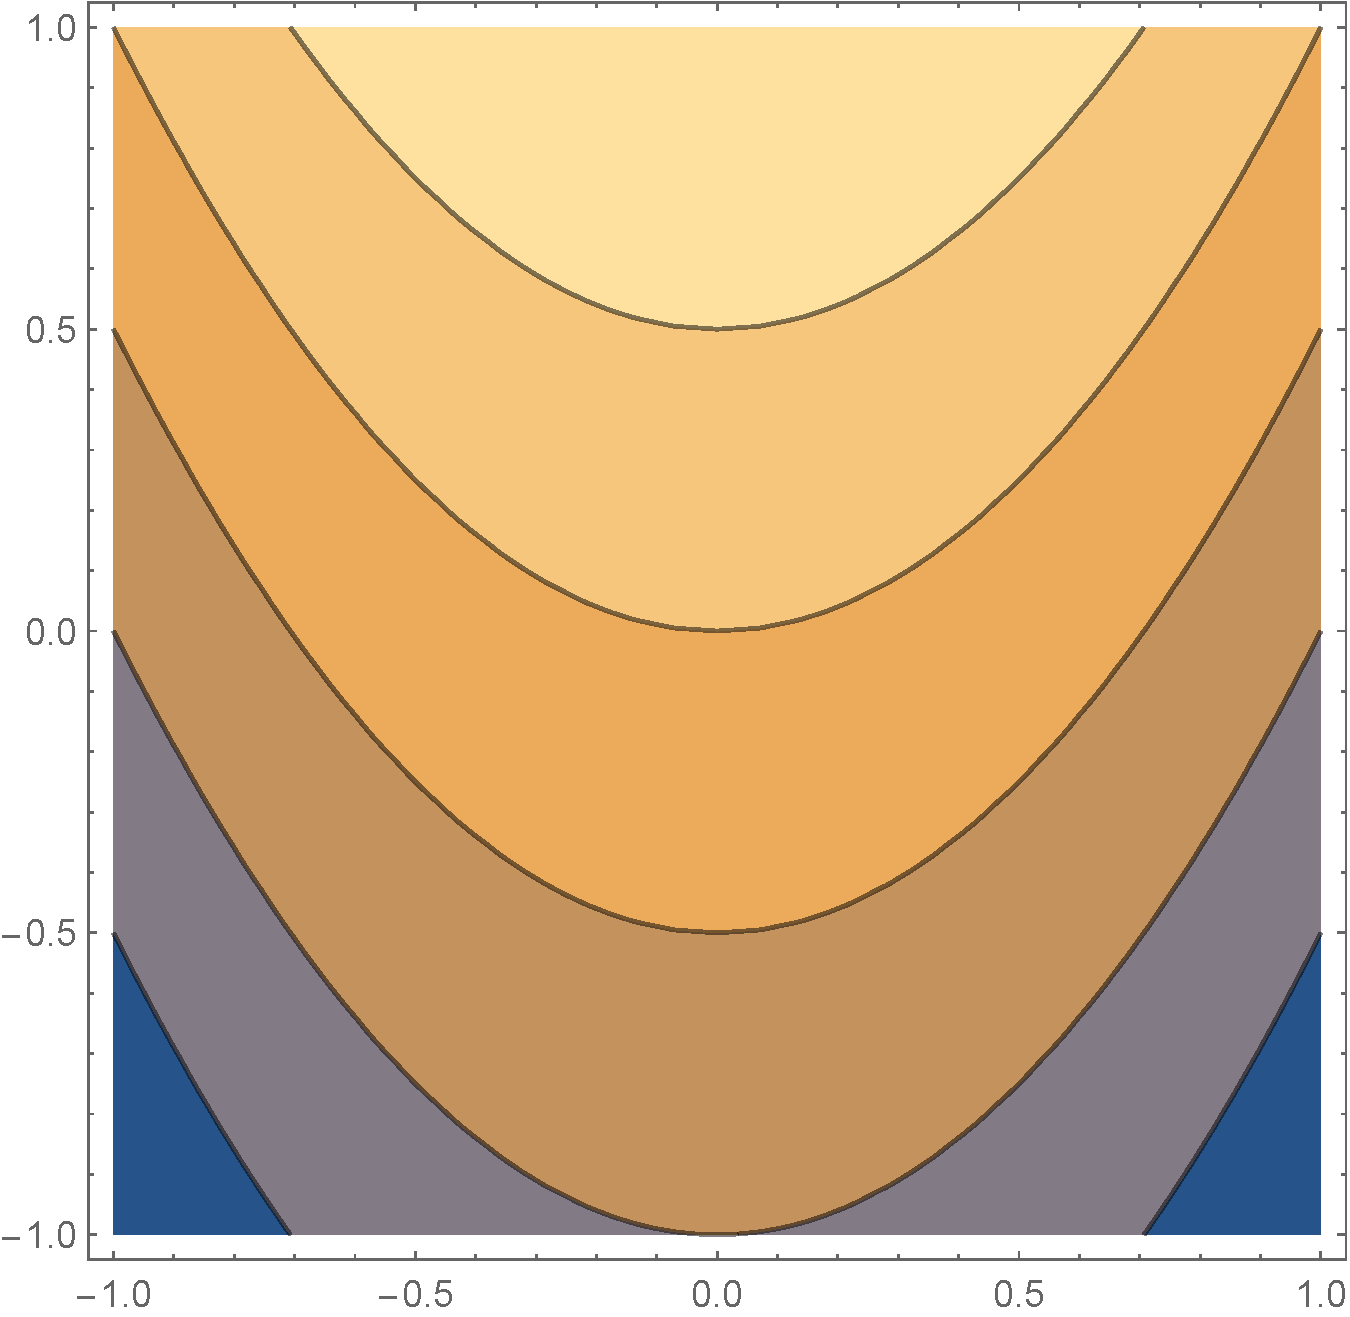
\includegraphics[scale=.27]{images/ContourPlot}
\end{figure}

	Afinal, o que foi feito para que chegássemos nessa conformação de curvas? A resposta é simples. Simplesmente assumimos que $f(x)=x^{2}$, trocamos $f(x)$ por $y$ e subtraímos $x^{2}$ de ambos os lados, logo
	
	\begin{equation}
		y-x^{2}=0
	\end{equation}
	
	Isso significa que temos um contorno da função $f$ cujo rótulo corresponde a 0. Ou seja, o valor nulo encontrado demonstra que a função $f$ ao longo de toda a curva $y-x^{2}$ está rotulado como 0 em três dimensões (Altura constante ao longo dessa parábola). Nesse caso, como estamos tratando de rótulos um atributo interessante de ser usado é o \ttt{ContourLabels}. Ele vai mapear a altura de cada parábola na representação em duas dimensões. Vejamos
	
\begin{lstlisting}[language=Mathematica]
ContourPlot[y - x^2, {x, -1, 1}, {y, -1, 1}]
\end{lstlisting}

	\begin{figure}[!h]
		\centering
		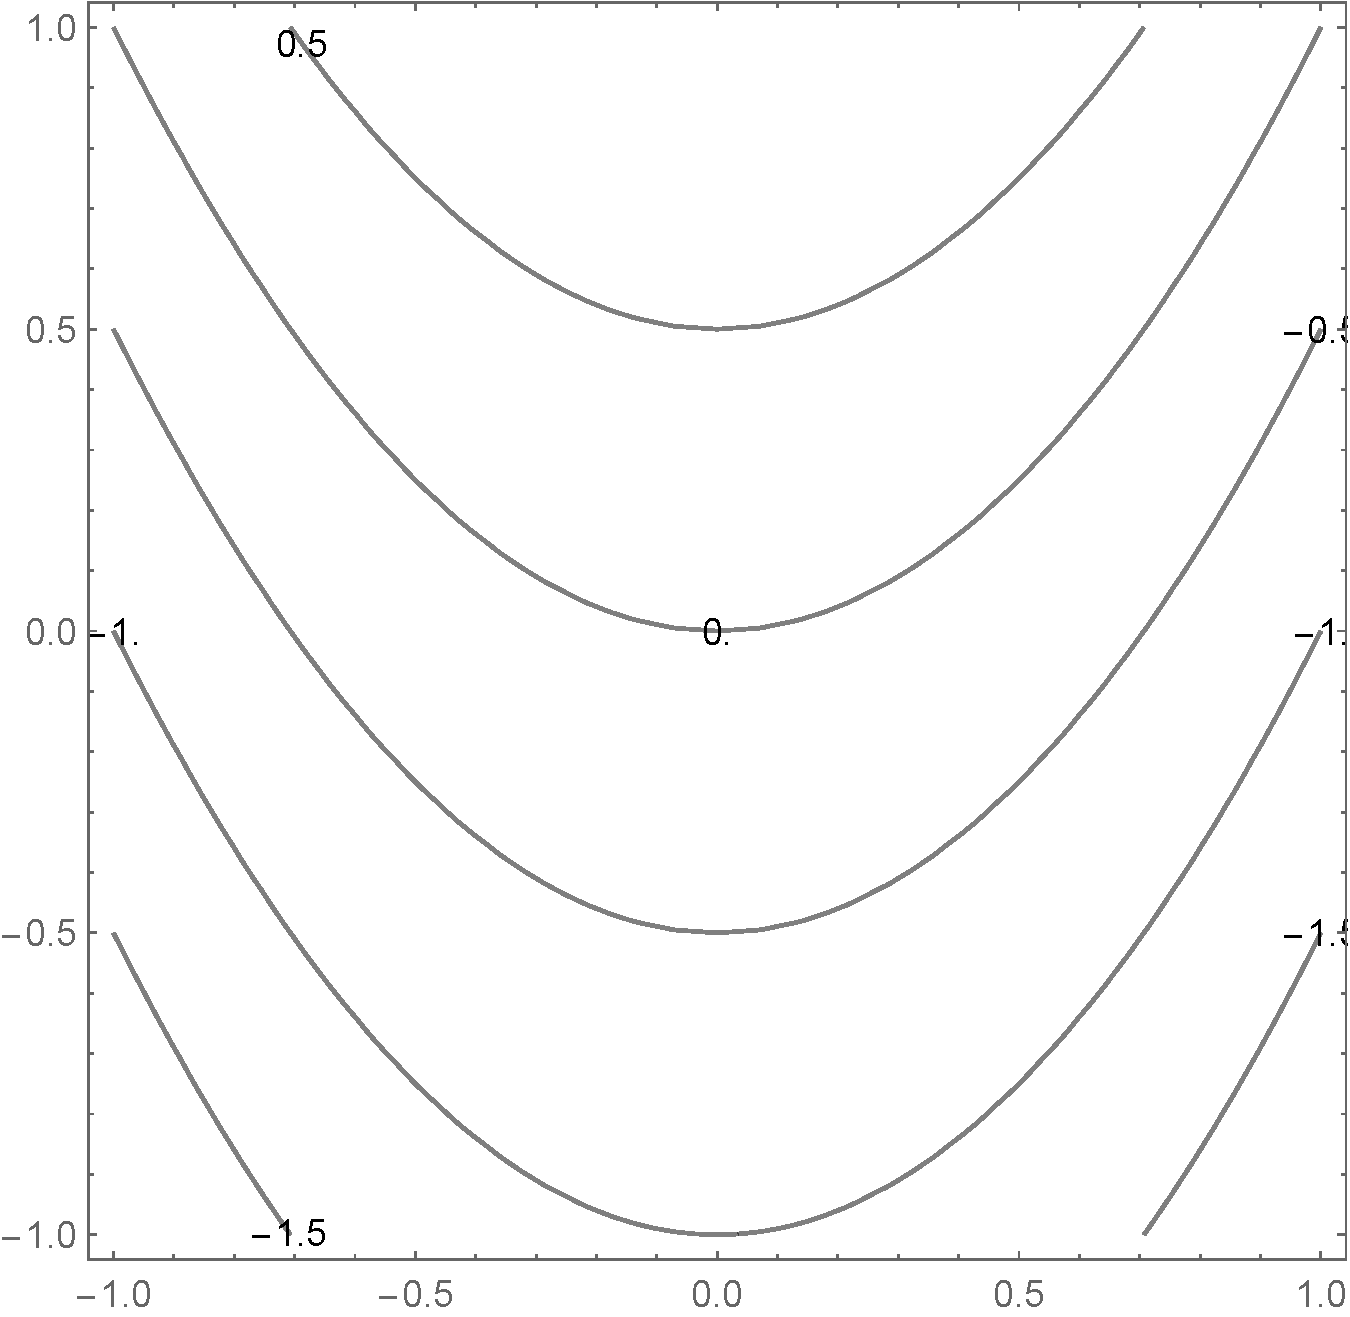
\includegraphics[scale=.47]{images/ContourLabels}
	\end{figure}

	Vemos o mapa de contornos referido. Para melhorar a visualização empregou-se o \ttt{ContourShading->False}
\end{document}
















